\addtocontents{toc}{\protect\newpage}
\chapter{Kutatási eredmények}\label{ch:eredmenyek}

Ebben a fejezetben kutatási kérdésenként haladva összefoglalom kutatásom eredményeit. A \ref{genai-megiteles}. alfejezetben bemutatom a generatív mesterséges intelligenciával kapcsolatos általános vélekedéseket (\textbf{RQ1}). A \ref{genai-felhasznalas}. alfejezetben az SDLC fázisai szerint haladva áttekintem a generatív mesterséges intelligencia lehetséges felhasználásait  (\textbf{RQ2}), valamint a vonatkozó tapasztalatokat, kihívásokat és korlátokat (\textbf{RQ3}).

\section{A generatív mesterséges intelligencia megítélése}\label{genai-megiteles}

Ebben az alfejezetben a generatív mesterséges intelligenciával kapcsolatos általános vélekedéseket összegzem, vagyis az \textbf{RQ1} kutatási kérdést vizsgálom: \emph{Hogyan vélekednek a szoftverfejlesztésben dolgozók általánosságban a generatív mesterséges intelligenciáról?}

\paragraph{Újdonság varázsa.} A generatív mesterséges intelligenciát körülövezi az újdonság varázsa. Sokan izgalmasnak tartják a technológiát és szeretnek kísérletezni vele, vagyis a használata nemcsak a hatékonyságra, hanem az általános fejlesztői közérzetre (wellbeing) is jó hatással lehet \parencite{McKinseyDevProd}. Az újdonság varázsa ugyanakkor nem tart örökké, és a sikertelen használat (pl. sok körös ismételt promptolás egy hiba javításáért) frusztráló is tud lenni, ahogyan az is, ha egy szervezeten belül túlságosan erőltetik az MI használatát.

\paragraph{Átalakuló munkakörök.} A megkérdezettek általánosságban nem féltik a munkájukat, azt gondolják, továbbra is szükség lesz szoftverfejlesztői és szakterületi tudással rendelkező emberekre, de a munkakörök átalakulása már most elkezdődött \parencite{DeloitteQuality}. Aki nem használ AI-t, nem lesz versenyképes, így kulcsfontosságú a tanulási képesség, pl. a helyes promptok megfogalmazásához (prompt engineering). Egyelőre nem alakult ki iparági konszenzus azt illetően, hogyan hat majd az MI a szükséges fejlesztői létszámra: vannak, akik szerint a technológia fejlődés miatt még több szakemberre lesz szükség, míg mások szerint épp ellenkezőleg \parencite{McKinsey_state_AI}. Jelenleg az sem egyértelmű még, hogy ahol történtek már leépítések, ott valóban az MI használat sikere állt-e mögöttük, nem pusztán a korábbi túlzott bővülés korrekciója \parencite{HoldAIHypePodcast}.

\paragraph{Junior fejlesztők.} Egyre szélesebb körben terjed az a vélekedés, hogy a junior fejlesztőknek nem szabad engedni a generatív MI eszközök használatát. A vonatkozó érvelés szerint a tudás akkor rögzül igazán, amikor mi magunk jövünk rá a megoldásra, akkor nem, ha megmondják nekünk. Vagyis maga a gondolkodás, a megoldás keresése, a ,,szenvedés’’ rögzíti a tudást\footnote{Az alapszakos egyetemi tanulmányaim legelején elsőként kezembe került jegyzet \parencite{bsz1} előszava idézte az anekdotát, amely szerint amikor I. Ptolemaiosz király megkérdezte Euklidészt, a kor nagy matematikusát, hogy nem lehetne-e a geometriát az Elemek \parencite{Elemek} áttanulmányozásánál könnyebben elsajátítani, Euklidész azt válaszolta: „A geometriához nem vezet királyi út. [...] Munka nélkül nincs kenyér, sem geometria.”} – ami nélkül egy hasonló, de nem pontosan ugyanolyan problémát már nem fogunk tudni megoldani. Rövid távon ugyanakkor más a helyzet, hiszen a legnagyobb produktivitásnövekedést pont a junioroknál okozzák a generatív MI eszközök \parencite{GithubCopilotProductivity}. Létező vélekedés az is, hogy az MI teljesen kiváltja a junior fejlesztőket, kérdés ugyanakkor, hogy a jelen junior fejlesztői nélkül kik lesznek a jövő senior fejlesztői.

\paragraph{Felesleges szóáradat.} A megkérdezettek közül többen is felvetették azt a nehézséget, hogy a generatív MI modellek feleslegesen hosszan fogalmazzák meg a válaszokat. Olyan ez, mintha ezt az új technológiát a nem hatékony emberi kommunikációhoz igazítanánk, ami olyan abszurd helyzetekhez vezethet, hogy egy MI modell által hosszasan megfogalmazott szöveget egy másik MI modellel foglaltatnak össze, holott semmi garancia nincs arra, hogy eközben nem torzul az eredeti információ. 

\paragraph{Kreativitás hiánya.} Mivel az MI modelleket a meglévő adatokon tanítják, sokak szerint nem lehetnek képesek igazi kreativitásra, valóban újszerű megoldások megalkotására (out of the box thinking). Vannak, akik szerint az embert valójában az \textit{absztrahálás} képessége tette naggyá, és erre az MI igazán sosem lesz képes.

\paragraph{Kilátások.} Azt illetően egyetértés uralkodik a megkérdezettek között, hogy a generatív MI az elmúlt években hatalmasat fejlődött. Arról ugyanakkor már megoszlanak a vélemények, hogy mi várható a jövőben: vannak, akik a fejlődés további gyorsulását várják, míg mások lassulásra számítanak a hatalmas energiaigény és a valós tanító adatok kimerülése miatt.

\section{A generatív mesterséges intelligencia felhasználása}\label{genai-felhasznalas}

Ebben az alfejezetben bemutatom a generatív mesterséges intelligenciával szoftverfejlesztésbeli felhasználhatóságát, valamint áttekintem az azokat övező tapasztalatokat, kihívásokat és korlátokat, vagyis az \textbf{RQ2} (\emph{Hogyan használható a generatív mesterséges intelligencia a szoftverfejlesztési életciklus (SDLC) különböző fázisaiban?}) és \textbf{RQ3} (\emph{A tapasztalatok alapján mik a generatív mesterséges intelligencia szoftverfejlesztésbeli felhasználásának kihívásai és korlátai?}) kutatási kérdéseket vizsgálom. Először általános megállapításokat fogalmazok meg, majd a továbbiakban az SDLC fázisai mentén mutatom be az eredményeket.

\paragraph{Emberi kontroll.} \textit{,,Lustaságból használni jó, tudatlanságból használni veszélyes’’} – foglalja össze a generatív mesterséges intelligenciában (nagy nyelvi modellekben) rejlő lehetőségeket és az azokat övező veszélyeket \emph{Egyetemi docens 1.}, rámutatva ezzel a hallucináció problémájára, és arra, hogy mennyire veszélyes vakon megbízni az MI által generált válaszokban. Mivel a modellek esetenként helyesnek tűnő, de valójában teljesen hibás válaszokat adnak, elengedhetetlen az emberi utóellenőrzés, amelyhez emberi tudásra van szükség. Iparági ajánlások is felhívják a figyelmet az MI emberi kontrolljának fontosságára \parencite{GartnerProdBoost}.

\paragraph{Specifikusság, pontosság.} A generatív mesterséges intelligencia számos olyan fejlesztési feladat megoldására használható, amelyekre már korábban is léteztek kizárólag algoritmikus (a mai köznyelv MI meghatározása alapján „MI-mentes”) megoldások. Jelentős különbség, hogy az algoritmikus módszerek determinisztikusak, belső működésük pontosan leírható, így eredményük is megmagyarázható, helyességük pedig bizonyítható. Ezek az eszközök tehát biztonságosan használhatók, cserébe csak egy-egy konkrét részfeladatot képesek megoldani. Ezzel szemben a generatív MI alapú eszközök belső működésüket tekintve \textit{fekete dobozok (black box)}, azaz nem tudjuk megmagyarázni, az adott bemenetre miért pont az adott kimenetet adják. A belső működés átláthatatlansága bizonytalanságot és pontatlanságot hordoz, cserébe ezek az eszközök univerzálisak, hiszen különböző jellegű kérdésekre egyaránt adnak \textit{valamilyen} választ. A problémák orvoslására megjelentek a generatív MI-t használó specifikus céleszközök, amelyek az univerzalitás feláldozásáért cserébe pontosságot ígérnek. Fontos látni, hogy a dilemma valójában a pontosság (feladatspecifikus eszköz, biztosan helyes eredmény) és a kényelmesség (univerzális eszköz, bizonytalan eredmény) között húzódik, az igazi áttörést pedig az olyan integrált eszközök jelentenék, amelyek \textit{megbízhatóan} képesek támogatni a teljes szoftverfejlesztési folyamatot \parencite{mckinsey2025aipdlc}.

\paragraph{Megspórolt idő.} A generatív mesterséges intelligencia potenciálisan hatékonyabbá teszi a szoftverfejlesztést, vagyis a fejlesztők bizonyos feladatokat rövidebb idő alatt tudnak elvégezni, mint korábban. Mivel így kevesebb időt kell egyes technikai részekkel eltölteniük, több idejük marad magasabb szintű tervezésre, munkatársakkal együtt gondolkodásra, új technológiák elsajátítására \parencite{github_genai_devtime}.

\paragraph{Kódoláson túl.} A technológia felhasználásának fókuszában a kódolás áll \parencite{Gartner_AICodeAssistants_2025}, amit a panelbeszélgetések során elhangzott ötletek eloszlása is alátámaszt (\ref{fig:sdlcbrainstorming}. ábra). Fontos azonban látni, hogy a szoftverfejlesztők valójában a munkaidejük jóval kisebb részét töltik kódolással, mint azt akár ők, akár a menedzsereik gondolják \parencite{SoftwareCom_CodeTimeReport, today_was_a_good_day}. Éppen ezért a kódolási asszisztensek produktivitásnövelő hatása a teljes szoftverfejlesztési folyamatra vetítve nagyon korlátos. Olyan eszközökre van szükség, amelyek a generatív mesterséges intelligencia segítségével az SDLC valamennyi fázisát hatékonyabbá teszik \parencite{gartner_ai_sdlc}.

\begin{figure}
	\centering
	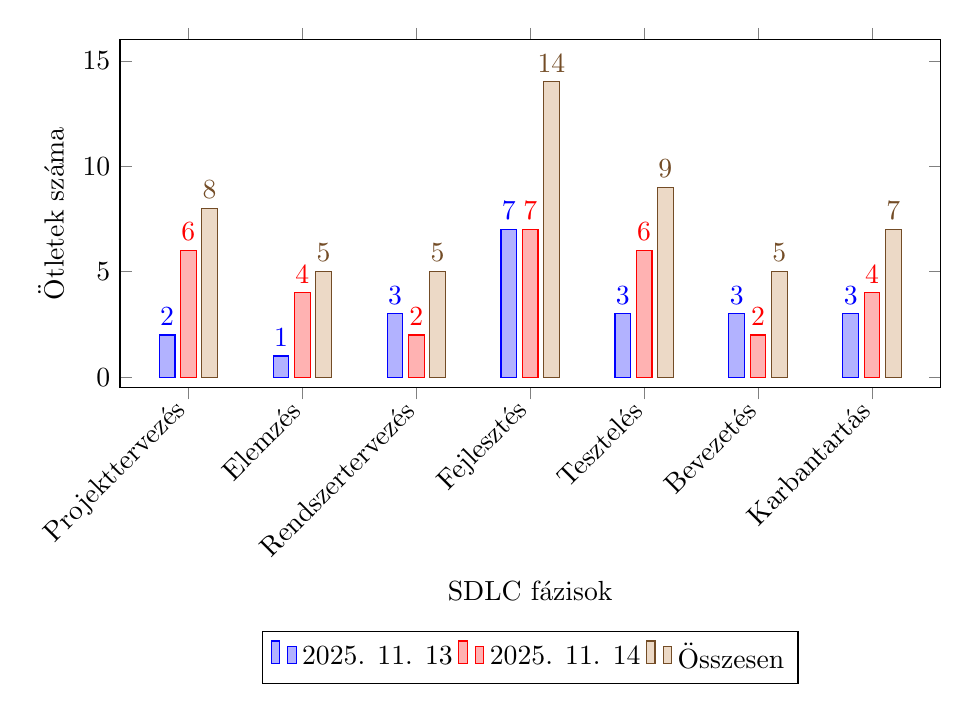
\begin{tikzpicture}
		\begin{axis}[
			xlabel={SDLC fázisok},
			ylabel={Ötletek száma},
			ybar,
			bar width=0.2cm,
			width=12cm,
			height=6cm,
			ymax=16,
			legend style={at={(0.5,-0.7)}, anchor=north, legend columns=3},
			xtick={1,2,3,4,5,6,7},
			xticklabels={Projekttervezés, Elemzés, Rendszertervezés, Fejlesztés, Tesztelés, Bevezetés, Karbantartás},
			x tick label style={rotate=45, anchor=east},
			ylabel near ticks,
			nodes near coords,
			]
			
			\addplot coordinates {(1,2) (2,1) (3,3) (4,7) (5,3) (6,3) (7,3)};
			\addlegendentry{2025. 11. 13}
			
			\addplot coordinates {(1,6) (2,4) (3,2) (4,7) (5,6) (6,2) (7,4)};
			\addlegendentry{2025. 11. 14}
			
			\addplot coordinates {(1,8) (2,5) (3,5) (4,14) (5,9) (6,5) (7,7)};
			\addlegendentry{Összesen}
		\end{axis}
	\end{tikzpicture}
	\caption{A panelbeszélgetéseken elhangzott ötletek eloszlása SDLC fázisok szerint. (Saját szerkesztés.)}
	\label{fig:sdlcbrainstorming}
\end{figure}

\subsection{Projekttervezés}

A projekttervezés során határozzuk meg a szoftverprojekt célját, hatókörét, erőforrásait és kockázatait. Másképp megfogalmazva meg kell határoznunk, hogy \textit{mit} (cél, hatókör) és \textit{mivel} (erőforrások, kockázatok) fogunk csinálni. Noha a szakirodalom kevés konkrét, valós felhasználási esetet említ ebből a fázisból, a megkérdezettek a jövőbe tekintő spekulációk mellett beszámoltak konkrét tapasztalatokról is, jóllehet, azok gyakran inkább még csak kísérletezésnek tekinthetők.

\paragraph{Helyzetfelmérés.}
A projekttervezés első lépése rendszerint az aktuális helyzet feltérképezése, amely egyaránt jelentheti a szervezet belső működését és a külső környezetet. A belső működés kapcsán fel kell mérni a használt folyamatokat, a meglévő rendszereket, azok főbb komponenseit, valamint a mindezek közt húzódó kapcsolatokat. A küldő környezetnek meghatározó elemei többek között a versenytársak és a szabályozók. Mindezekről rendszerint sokféle, töredezett, heterogén információ áll rendelkezésre, amelyek feldolgozása és összegzése időigényes emberi feladat. A GMI ugyanakkor hatékonyan képes feldolgozni és összefoglalni az ilyen széttagolt tudáshalmazokat.

A GMI ez irányú hatékony használatához elengedhetetlen a belső vállalati működést leíró dokumentumok beemelése a modell kontextusába. Mivel ezek általában érzékeny üzleti adatokat tartalmaznak, felmerülnek adatvédelmi aggályok az adatok sorsát illetően \parencite{CopilotingFuture}. Amennyiben az adatok nem oszthatók meg az MI modellel, az nagyban korlátozza a hatékonyságot. Megoldás lehet az is, ha egy vállalat saját maga futtat on-premise MI modellt, de ennek komoly hardverberuházási költsége van (a nagyméretű modellek futtatásához olyan nagy hardverkapacitásra van szükség, amelyet egyetlen vállalat reálisan nem tud hatékonyan kihasználni). Ennek alternatívája, amikor a modellek virtuális privát felhőben futnak, vagyis a hardvert nem kell megvásárolni, mégis biztonsági mechanizmusok gátolják meg a vállalati adatok kiszivárgását.

\paragraph{Brainstorming.} A projekttervezés potenciális eleme az ötletgyűjtés, vagyis a lehetséges fejlesztési irányok, megoldások, kiegészítő funkciók összegyűjtése. A brainstorming célja nem a mély technikai elemzés, hanem a lehetőségek minél sokszínűbb feltérképezése. A generatív MI ebben kifejezetten hatékony, hiszen képes a megadott célok és korlátok mentén nagyszámú ötletet és hivatkozást összegyűjteni.

Az ilyen típusú ötletgenerálás különösen hasznos akkor, amikor a projekt kezdeti szakaszában „vakfoltok” merülhetnek fel, illetve amikor a csapatnak nincs kellő kapacitása szisztematikus kutatásra. Fontos ugyanakkor kiemelni, hogy a GMI nem helyettesíti a mély domain-szakértelmet, inkább csak széleskörű, de gyakran felszínes irányokat tud mutatni, amelyek közül már az emberi tudás és intuíció alapján érdemes választani.

\paragraph{Értékelés.} Az ötletelést követően elengedhetetlen az egyes koncepciók részletes értékelése, vagyis annak vizsgálata, hogy az adott javaslat mennyire életképes, milyen előnyei és hátrányai vannak, illetve milyen hozzáadott értéket képvisel. Ebben a lépésben a GMI képes strukturált érveket generálni (pro-kontra listák), rámutatva ezáltal olyan szempontokra, amelyek a fejlesztőcsapat számára elsőre nem kézenfekvőek, különösen, ha a csapat összetétele nem fedi le az összes releváns szakterületet. A panelbeszélgetések résztvevői is megemlítették, hogy a modellek gyakran váratlan, de releváns szempontokat hoznak fel egy adott ötlettel kapcsolatban.

Az értékelés fontos része lehet a rendelkezésre álló adatokra épülő elemzés is, pl. hogy egy új funkciót valóban használna-e a felhasználói bázis. A GMI képes rövid szöveges összefoglalókat generálni nagy mennyiségű analitikai adatból és felhasználói visszajelzésből, ezzel hatékonyan támogatva a döntés-előkészítési folyamatot. Ennek a felhasználásnak természetesen előfeltétele, hogy megfelelő mennyiségű és minőségű adat áll rendelkezésre, amelyekből az MI modell dolgozni tud. Általánosságban is elmondható, hogy adat nélkül hatékony MI használat sincs.

\paragraph{Kockázatelemzés.} A projekttervezés során elengedhetetlen a kockázatok feltárása. A potenciális kockázatok tárháza szinte végtelen: technológiai, erőforrásbeli, üzemeltetési, biztonsági vagy megfelelőségi (compliance) kockázatokra egyaránt fel kell készülni. A GMI ebben a szakaszban jó kiegészítő eszköz lehet, hiszen rengeteg korábbi példát, iparági esetleírást, legjobb gyakorlatot (best practice) és dokumentációt használtak fel a modell tanítása során, amelyekből kiindulva képes lehet releváns kockázatokat azonosítani.

Az MI modellek ugyanakkor egyelőre nem helyettesíthetik a szakértők munkáját, hiszen csak a múltbeli példákból és az azokon felismert mintázatokból tud dolgozni, holott a kockázatok kimerítő feltárása a gyakorlatban gyakran igényel kreativitást. Ráadásul az adott szervezet egyedi kontextusát sem szabad figyelmen kívül hagyni, amely nem biztos, hogy kimerítően beemelhető a modell kontextusába. A GMI tehát ebben a szakaszban inkább a gondolkodási horizont szélesítésében, mintsem a döntéshozatalban játszik szerepet.

\paragraph{Becslés.} Egy projekt sikeressége többek között az idő- és erőforráskeretek betartásában mérhető, amelyek alapja a reális idő- és erőforrásbecslés. A generatív MI erre is használható: a modell a meglévő kódbázis, az érintett komponensek, korábbi hasonló projektek és fejlesztői becslések alapján képes előzetes idő- és munkaigénybecslést kalkulálni \parencite{GenAISWEresearchAgenda}. A panelbeszélgetések során is említették, hogy egy új funkció fejlesztéséhez szükséges időt a specifikáció és a forráskód fontosabb részei alapján a GMI modellek képesek meglepően pontosan megbecsülni.

\paragraph{Dokumentumgenerálás.} A projekttervezés végső kimenete általában formális dokumentum, mint pl. projektterv, kezdeti specifikáció, követelménylista, kockázatelemzés vagy becslési táblázat. A generatív MI jelentősen felgyorsíthatja ezeknek a dokumentumoknak az előállítását. A modell képes a rendelkezésre álló adatok, feljegyzések, részeredmények alapján jól strukturált, koherens  dokumentumokat generálni, amelyek és formai szempontból illeszkednek korábbi referenciamunkákhoz \parencite{Oracle2024_GenerativeAI_SoftwareDevelopment}.

A gyakorlatban ez nemcsak időt takarít meg, hanem javíthatja a dokumentumok minőségét is, mivel a modell képes konzisztens terminológiát, egységes szerkezetet és átlátható formátumot biztosítani. Ugyanakkor fontos látni, hogy a generált dokumentumokat minden esetben emberi utóellenőrzésnek kell alávetni, különösen tartalmi szempontból, hiszen a projekt további sikeressége szempontjából elengedhetetlen a pontosság garantálása.

\subsection{Elemzés}

Az elemzés során határozzuk meg és dokumentáljuk a szoftverrel szemben támasztott követelményeket. A követelmények célja, hogy a projekt minden résztvevője számára teljesen egyértelmű legyen, hogy a készítendő megoldásnak pontosan mire kell \textit{képesnek lennie} (funkcionális követelmények) és \textit{milyennek} kell lennie, vagyis milyen minőségi jellemzőkkel kell rendelkeznie a megoldásnak (extrafunkcionális követelmények). MI alapú követelményelemző eszközök léteznek ugyan a gyakorlatban is, de a GMI ilyen irányú felhasználása egyelőre inkább tűnik jövőbeli elképzelésnek, mint múltbeli gyakorlatnak.

\paragraph{Követelményszármaztatás.} A követelmények jelentős része származhat különböző dokumentumokból, amelyek tartalmát adottságként kell kezelni. Ezek egyaránt lehetnek belső vállalati (pl. illesztendő meglévő rendszerek tulajdonságai, belső információbiztonsági szabályzatok) és vállalaton kívüli (pl. szabályozói előírások – különösen szigorúan szabályozott nagyvállalati környezetben) források. A GMI képes lehet kinyerni ezekből a forrásokból a lényeges információkat, majd strukturálni és formális követelményekké alakítani azokat \parencite{rico2025challenges}, vagy pontosítani a már meglévő követelményeket, esetleg rámutatni hiányzó követelményekre. Az MI modell felismeri a követelményként értelmezhető mondatokat, és képes azokból egységes szerkezetű, pontos követelményeket származtatni. Ez különösen hasznos olyan projekteknél, ahol nagy mennyiségű kiinduló forrás tartalmaz potenciális követelményeket, ezek a források pedig heterogének, eltérő formátumúak.

Fontos ugyanakkor rámutatni, hogy egy szoftverprojekt szempontjából a követelmények összegyűjtése kritikus fontosságú. Ennek a fázisnak a precizitásán nagyban múlik a később szükséges iterációk száma, így az MI által származtatott követelményeket mindenképp szükséges emberi utóellenőrzés alá vetni. Kritikus fontosságú továbbá a követelmények teljességének az ellenőrzése, vagyis a megbizonyosodás arról, hogy valóban minden releváns követelmény összegyűjtésre került.

\paragraph{Követelményosztályozás.} A követelményeket általában osztályozzuk a jellegük szerint, vagyis az alapján, hogy mire vonatkoznak. Beszélhetünk funkcionális és extrafunkcionális követelményekről, utóbbi kategórián belül többek között teljesítményre, megbízhatóságra, biztonságra, megfigyelhetőségre, kompatibilitásra, karbantarthatóságra, használhatóságra vonatkozó követelmények. A GMI segíthet az elkészült követelmények osztályozásában \parencite{GenAISWEresearchAgenda}, ami elősegíti a rendezett követelménystruktúrát, és átláthatóbb dokumentációt eredményez.

\paragraph{Követelményminőség.} Bár a követelmények természetes nyelven kerülnek megfogalmazásra, a későbbiekben viszont egzaktan kell tudnunk ellenőrizni a megvalósulásukat, ezért kritikus fontosságú a precíz megfogalmazás. Ennek biztosítására különböző szabályok léteznek a megfogalmazására, amelyek célja a követelmények egyediségének, azonosíthatóságának, egyértelműségének és tesztelhetőségének biztosítása. Kerülni kell tehát a túl általános, homályos, félreérthető megfogalmazásokat, amelyekről nem dönthető el egyértelműen, hogy megvalósultak-e. A nagy nyelvi modellek képesek lehetnek ellenőrizni ezeket a megfogalmazásbeli elvárásokat, különösen, ha az elvárások minél részletesebben megfogalmazva állnak rendelkezésre.

\paragraph{Megvalósíthatóság.} A követelmények összegyűjtése után meg kell vizsgálni, hogy azok megvalósíthatók-e. A megvalósíthatóság több síkon is értelmezhető, mint pl. technikailag, üzletileg és erőforrások szempontjából. A megvalósíthatóság szükséges, de nem elégséges alapfeltétele a követelmények ellentmondás-mentessége. A generatív MI segíthet a potenciális ellentmondások, egymással nem összhangban lévő követelmények azonosításában, ami főleg nagy számú/terjedelmű követelmények esetében lehet különösen hasznos. A modellek akár képesek is lehetnek megoldási javaslatokat tenni az ellentmondások feloldására. Ugyanakkor az értelmezés és döntéshozatal továbbra is emberi feladat, hiszen a megvalósíthatóság végső megítélése mély szakterületi tudást igényel.

\subsection{Rendszertervezés}

A rendszertervezés során definiáljuk a rendszer logikai és technikai architektúráját, az adatmodelleket, valamint a komponensek közti kapcsolatokat és interfészeket. Gondos tervezéssel lehetséges az esetleges hibák korai feltárása, ami nagyban elősegíti a későbbi folyamatok (különösen a fejlesztés és a tesztelés), így összességében az egész SDLC hatékonyságát. A megkérdezettek tapasztalatai alapján a részletes rendszertervezést nem adják ki emberi kézből, de prototípusok generálására már most is aktívan használják a GMI-t.

\paragraph{Technológiaválasztás.} A technológiaválasztás során a fejlesztőcsapatnak meg kell határoznia, hogy a projekt mely eszközökre, keretrendszerekre, könyvtárakra és infrastruktúrára támaszkodik. Mivel vállalati környezetben a rendszerek jellemzően hosszútávra készülnek, a kiválasztás során nemcsak a jelen körülményeit kell figyelembe venni, hanem azt is, hogy a választott technológiák támogatása hosszútávon biztosított-e. Sőt, az is fontos mérlegelési szempont lehet, hogy mennyire közismert a technológia, hiszen ez közvetlenül befolyásolja, hogy mennyire könnyen (és milyen költségen) lehet fejlesztőt találni a projektre. A generatív MI képes lehet feltérképezni a potenciális megoldásokat (ideértve a \textit{state of the art}-ot is), összefoglalni a főbb előnyöket és hátrányokat, és mindezek alapján javaslatokat megfogalmazni \parencite{CopilotingFuture, rico2025challenges}. Ezek az ötletek segíthetnek ugyan a döntéshozók perspektívájának tágításában, de az MI modell javaslatainak kritikátlan felhasználása helyett nem szabad szem elől téveszteni a döntések súlyát, hiszen a technológiaválasztás hosszútávú következményekkel járhat az üzemeltetésre, a teljesítményre, a biztonságra és a bővíthetőségre nézve.

\paragraph{Prototipizálás.} A rendszertervezés fontos támogató tevékenysége a prototípusok készítése, amelyek célja a koncepciók gyors validálása és a magas szintű megoldási irányok gyakorlati kipróbálása. A generatív MI ebben a fázisban képes gyorsan létrehozni egyszerű proof-of-concept (PoC) vagy minimális életképes termék (minimal viable product, MVP) jellegű megoldásokat, beleértve az alapvető infrastruktúra-komponenseket vagy egyszerű felhasználói felületeket. Ez jelentős időmegtakarítást eredményezhet, különösen akkor, ha a projekt több lehetséges architektúrát is vizsgál, lehetővé téve azok összehasonlítását. Az összehasonlításon túl ez a módszer egy új technológia megismerésekor is hasznos lehet, hiszen egy egyszerű, ám mégis működő példán keresztül sokszor könnyebben elsajátítható az új tudás. Fontos azonban hangsúlyozni, hogy a prototípusokat a helyükön kell kezelni, azok semmiképp sem tekinthetők végleges terveknek. Az MI modellek által generált kód és architektúra sok esetben csak demonstrációs célokra alkalmas, és az sem garantált, hogy hűen reprezentálja az adott technológia használhatóságát.

\paragraph{Tervezés.} A GMI képes lehet egyszerűbb komponensek konkrét megtervezésére is, mint pl. egy egyszerű API (application programming interface, a szoftverkomponensek közti kommunikáció interfésze), valamint a vonatkozó metrikák (pl. szükséges tárhely, memória, sávszélesség) becslésében is segítséget nyújthat. Fontos azonban kiemelni, hogy még ha elsőre hívogatónak is tűnhet egy komplett rendszerterv legenerálása, valójában nagyon veszélyes. Egy komplex rendszerterv, különösen a hozzá kapcsolódó dokumentációk olyan összetettek és terjedelmesek, hogy azoknak a kellően tüzetes emberi utóellenőrzése egész egyszerűen irreális. A megkérdezettek ráadásul egyetértettek abban, hogy egy nem általuk készített komplex megoldás kellő részletességű átnézése valójában gyakran nehezebb és nagyobb szellemienergia-befektetést igényel, mint ha ők maguk készítették volna el, így pedig nagyon könnyű átsiklani az MI által vétett hibák felett.

\subsection{Fejlesztés}

A fejlesztés során ténylegesen implementáljuk a szoftvert, vagyis megvalósítjuk a rendszertervet. A megvalósításnak teljesítenie kell a korábban meghatározott követelményeket. Ebben a fázisban általában többnyire kódolás zajlik, amely eredményeként előáll a szoftver forráskódja. A GMI alkalmazása itt a legkézenfekvőbb és legelterjedtebb, amit több dolog is alátámaszt: egyrészt ehhez a fázishoz áll rendelkezésre a legtöbb GMI céleszköz, másrészt ezt (és a tesztelést) taglalja a legtöbb publikáció, harmadrészt a megkérdezetteknek is a kódolást illetően volt a legtöbb ötlete és tapasztalata.

\paragraph{Kódgenerálás.} A GMI kódgenerálásra (természetes nyelvi utasításokból programkód előállítása) való felhasználása jelentős időmegtakarítást eredményezhet, különösen a kevés tényleges gondolkodást igénylő, repetitív feladatok esetében. Ilyenek lehetnek többek között sablon (boilerplate) kódok, integrációs megoldások vagy a felhasználói felület (user interface, UI) egyszerű komponensei. A tapasztalatok szerint minél kevésbé komplex a feladat, annál hasznosabb a GMI, összetett üzleti logika vagy komplex technikai megoldások esetén viszont a modellek gyakran hibás vagy félrevezető kódot generálnak, és a javítás (vagy a modell rábírása a javításra) több erőfeszítést igényel, mint az önálló megírás \parencite{AI_pairprog, McKinseyDevProd, GenAITransformSWD}. A panelbeszélgetések résztvevői úgy foglalták össze ezt a jelenséget, hogy komplex esetekben hiába kezdik el lelkesen használni az MI-t a gondolkodás megspórolására, végül általában kiderül, hogy az \textit{igazán} bonyolult problémák végiggondolása, vagyis az \textit{igazi} gondolkodás nem spórolható meg.

A GMI-alapú kódgenerátorok alkalmazhatósága szempontjából kulcskérdés az adott szoftverkomponens szerepe: mivel a kódba kerülhetnek nehezen észrevehető hibák, a kevésbé fontos, nem kritikus részeken érdemes alkalmazni a technológiát. Azt is érdemes szem előtt tartani, hogy programnyelvenként eltérő garanciák vannak arra vonatkozóan, hogy milyen hibák milyen korán derülnek ki: míg egyes nyelvek lehet, hogy már le sem fordulnak, bizonyos szkriptnyelvek esetén elképzelhető, hogy csak jóval a bevezetés után, élesben derül majd fény egy hibára.

\paragraph{Megmagyarázás.} A generatív MI jól használható a meglévő kódrészek megértésének támogatására, ami különösen fontos nagy, rosszul dokumentált kódbázisok esetén. A modell képes összefoglalni, hogy egy adott függvény, osztály vagy modul mi célt szolgál, milyen bemeneteket és kimeneteket kezel, milyen kapcsolatban áll más komponensekkel, és mi a szerepe az egész rendszerben. Ez nagyban gyorsíthatja a fejlesztők munkáját, különösen új belépők vagy a projektbe frissen bekapcsolódó fejlesztők számára. A GMI megmagyarázó képessége újonnan írt kódok esetén is használható, többek között az új forráskód kommentezésével (kód ellátása magyarázó megjegyzésekkel) vagy a változások összefoglalásával (pl. verziókezelő számára).

\paragraph{Refaktorálás.} Refaktorálásnak nevezzük egy programkód átalakítását, a viselkedés módosítása nélkül, pusztán azért, hogy javuljon a kód struktúrája, olvashatósága, karbantarthatósága. A GMI hatékonyan támogathatja kisebb, jól körülhatárolt refaktorálási feladatok elvégzését, mint pl. változóátnevezés, kisebb logikai letisztázások, duplikációk eltávolítása, függvények szétbontása. Nagyobb léptékű, átfogó módosítások esetén azonban komoly kockázatot jelent, hogy a modell által generált változtatások olyan nagyok, hogy a fejlesztők már nem látják át teljesen, így végül vakon megbíznak az MI modellben. Ez magában hordozza a viselkedés akaratlan módosítását, ami olyan hibákat injektálhat a rendszerbe, amelyekre potenciálisan csak később, élesben derül fény. A megkérdezettek tapasztalatai is azt támasztották alá, hogy az MI által végzett refaktorálásokat mindenképp le kell ellenőrizni, mert könnyen végezhet nem várt, helytelen módosításokat is.

\paragraph{Hibakeresés.} A fejlesztési folyamat szerves részét képezi a készülő kód folyamatos kipróbálása és az iteratív hibakeresés, amelyben a generatív MI szintén nagy segítséget nyújthat. A modellek képesek értelmezni a kapott hibaüzeneteket, és a hibás kódban rámutatni a hibák tényleges okaira. A hibák szöveges magyarázatán túl képesek javaslatot tenni a javításra vagy akár konkrétan legenerálni a javított változatot. Ez még az egyszerű szintaktikai hibák esetén is hasznos lehet (pl. egy hosszú lekérdezésben könnyű apró hibákat véteni, amelyeket egyesével kijavítani jóval tovább tart, mint beadni az egészet az MI modellnek), de különösen hasznos, amikor a hiba valódi oka nem egyértelmű, egyszerűen csak egy váratlan viselkedésre keresünk magyarázatot.

\paragraph{Szkriptek.} A fejlesztés során gyakran adódnak olyan feladatok, amelyek nem tartoznak a fejlesztő szigorúan értelmezett szakterületéhez, de mégis meg kell őket oldania. Ez jelentheti akár bizonyos fejlesztői lépések automatizálását, akár adatok kinyerését fájlokból, a közös az bennük, hogy bár a feladatok egyszerűek, a praktikusan használt nyelvben (általában szkriptnyelv, pl. bash, awk) gyakran kevésbé magabiztos a fejlesztő, mert csak ritkán kényszerül használni. Ezek a feladatok tipikusan nem hordoznak jelentős kockázatot, és a generált megoldás is elég tömör és egyszerű ahhoz, hogy ,,ránézésre'' vagy első kipróbálásra megállapítható a helyessége, ugyanakkor jelentős időmegtakarítást eredményezhet, hogy nem kell egy kontextusváltás árán belemélyedni a ritkán használt nyelvbe. Bár nem szorosan tartozik ide, de mégis itt érdemes megemlíteni a reguláris kifejezések írását és értelmezését is, amiben szintén nagyon hasznos segítség lehet a GMI.

\paragraph{Konvertálás.} A fejlesztés során esetenként szükség van különböző fájlformátumok (pl. JSON, XML, CSV) közötti átalakításra, amit a GMI magabiztosan képes elvégezni. Az is előfordul, hogy egy adott programnyelven rendelkezésre álló logikát egy másik programnyelvben is elő kell állítani. Ez ugyan már jóval komplexebb feladat, mint egy fájlkonverzió, a tapasztalatok azt mutatják, hogy erre is használhatók a generatív MI modellek \parencite{GartnerAISWD, Oracle2024_GenerativeAI_SoftwareDevelopment}. A programnyelvek közti fordítás esetén is igaz, ami általánosságban is elmondható az MI által generált éles rendszerbe szánt kódokról: fontos megbizonyosodni a helyességről, akár emberi ellenőrzéssel, akár alapos teszteléssel.


\subsection{Tesztelés}

A tesztelés a szoftverfejlesztési életciklus kritikus fontosságú szakasza, melynek célja a szoftver minőségének biztosítása, a hibák feltárása, valamint annak igazolása, hogy az elkészült megoldás megfelel az előre meghatározott funkcionális és extrafunkcionális követelményeknek. A tesztelés hagyományosan erőforrásigényes és gyakran monoton tevékenység, amely azonban elengedhetetlen a későbbi, éles környezetben felmerülő, sokkal költségesebb hibák elkerülése érdekében. Mivel a tesztelés jelentős részét a tesztek megírása (kódolása) teszi ki, a fejlesztéshez hasonlóan itt is hatékony segítséget jelenthetnek a generatív MI megoldások. Ez a potenciál megmutatkozik a céleszközök és vonatkozó publikációk számában, és a megkérdezettek beszámolóiban is.

\paragraph{Tesztgenerálás.} A fejlesztők körében az egyik legnépszerűbb felhasználási mód a tesztek, különösen az egységtesztek (unit test) generálása (amely egy atomi funkcionális egység működését tesztelik). A GMI modellek képesek a forráskód alapján automatikusan teszteseteket írni, lefedve számos bemeneti kombinációt és végrehajtási ágat \parencite{PwC2024_GenAI_SWD_Improve, GenAITransformSWD}. Ez jelentősen növelheti a kódlefedettséget és csökkentheti a tesztírásra fordított időt.

Ugyanakkor fontos tisztában lenni egy súlyos módszertani korláttal: ha a teszteket a forráskódból származtatjuk (különösen, ha ugyanazzal a GMI modellel generáljuk őket, amely a forráskódot is generálta), az valójában \textit{fehér dobozos} tesztelést (white box testing) eredményez, ahol a tesztkészlet a kód belső működését tükrözi, nem pedig a specifikációt. Ha a kód hibás logikát vagy struktúrát tartalmaz, a generált tesztkészlet potenciálisan ehhez a hibás logikához fog illeszkedni, így hiába fut le sikeresen egy teszt, a tesztelni kívánt, de valójában nem tesztelt hiba mégis rejtve marad. A valódi minőségbiztosításhoz elengedhetetlen, hogy a tesztek a kódtól függetlenül, az elvárások (követelmények) alapján (is) készüljenek (\textit{fekete dobozos} tesztelés, black box testing).

\paragraph{Tesztadat-generálás.} A tesztelés során gyakori probléma a megfelelő minőségű és mennyiségű tesztadat előállítása. A valós éles adatok használata szigorú adatvédelmi és biztonsági kockázatokat vet fel, a kézi adatgyártás pedig lassú és nem skálázható. A generatív MI képes szintetikus, de a valós adatok statisztikai jellemzőit és struktúráját hűen tükröző tesztadatokat előállítani \parencite{PwC2024_GenAI_SWD_Improve}. Ez lehetővé teszi a fejlesztők számára, hogy biztonságosan teszteljenek határértékeket, kivételes eseteket vagy nagy adathalmazokat igénylő teljesítményteszteket végezzenek. Korlátot jelenthet ugyanakkor, hogy a generálás nem feltétlenül szisztematikus: a modell tanult minták alapján dolgozik, nem pedig algoritmikusan, így előfordulhat, hogy bizonyos speciális, de kritikus adatkombinációkat magától nem állít elő, hacsak a promptban erre külön nem utasítjuk.

\paragraph{Integrációs tesztelés.} Míg a unit tesztek a kód legkisebb funkcionális egységeit vizsgálják, az integrációs tesztelés a komponensek közötti együttműködés ellenőrzésére szolgál. Ez a terület komplexebb, mivel gyakran külső függőségeket, adatbázisokat vagy hálózati kommunikációt igényel. A fejlettebb, agentikus MI megoldások képesek lehetnek arra, hogy autonóm módon elindítsák a szükséges kódokat, felépítsék a tesztkörnyezetet, és szkriptek segítségével szimulálják és ellenőrizzék a komponensek közötti interakciókat \parencite{PwC2024_GenAI_SWD_Improve}. A GMI segíthet a komponenseket összekötő „ragasztó” kódok (glue code) és a teszteléshez szükséges konfigurációk elkészítésében is, ami jelentős terhet vesz le a tesztautomatizáló mérnökök válláról.

\paragraph{Kimenetellenőrzés.} A regressziós tesztelés során -- amikor azt vizsgáljuk, hogy egy módosítás nem rontott-e el korábban már működő funkciókat -- gyakran keletkeznek nagyméretű naplófájlok (logok) és kimeneti állományok. Ezek manuális átnézése rendkívül időigényes és az emberi figyelmet próbára tevő feladat. A generatív MI modellek hatékonyan használhatók a tesztfutások eredményeinek összehasonlítására. A modell képes összevetni az elvárt és a kapott kimenetet, kiemelni az eltéréseket, sőt, a hibaüzenetek alapján akár előzetes diagnózist is felállíthat a hiba lehetséges okáról, felgyorsítva ezzel a hibajavítási ciklust.

\paragraph{Kompatibilitásellenőrzés.} A szoftverek fejlődésének természetes velejárója a változás, azonban bizonyos helyzetekben fontos szempont a visszafelé kompatibilitás (backward compatibility) biztosítása, különösen API-k vagy mások (akár szervezete belül, akár azon kívül) által is használt könyvtárak esetén. A generatív MI segíthet a tervezett változtatások elemzésében, összevetve a régi és az új verzió interfészét és belső működését. A modell képes azonosítani azokat a módosításokat (pl. egy függvény szignatúrájának megváltozását vagy a belső működés nem kívánt megváltozását), amelyek problémát okozhatnának a szoftvert használóknál, még azelőtt, hogy a módosítás éles környezetbe kerülne.

\paragraph{Kódátvizsgálás.} A kódátvizsgálás (code review) kettős szerepet tölt be a GMI kontextusában. Egyrészt az ember által írt kód MI általi ellenőrzése értékes eszköz: a modellek \textit{fáradhatatlanul} képesek kiszűrni a szintaktikai hibákat, a biztonsági sérülékenységeket, vagy javaslatokat tenni a kód stílusának javítására \parencite{Oracle2024_GenerativeAI_SoftwareDevelopment, PwC2024_GenAI_SWD_Improve, GenAITransformSWD}, míg emberi ellenőrzés esetén számolni kellene a figyelem lankadásának veszélyével.

Másrészt viszont komoly kihívást jelent az MI által generált kód emberi felülvizsgálata. A kutatások és a gyakorlati tapasztalatok azt mutatják, hogy ha a kódot nagyrészt az MI generálja, az emberi fejlesztő hajlamos a felületes ellenőrzésre. Egyrészt pszichológiailag nehezebb és unalmasabb más (vagy egy gép) kódját olvasni és értelmezni, mint sajátot írni. Másrészt az MI által generált kód szintaktikailag általában helyes és „szépnek” tűnik, ami hamis biztonságérzetet ad. Így a fejlesztők könnyen átsiklanak olyan logikai vagy szemantikai hibák felett, amelyeket saját kódolás közben nem vétettek volna el, vagy azonnal észrevettek volna. Paradox módon tehát az MI által generált kód ellenőrzése esetenként nagyobb kognitív terhelést és fegyelmet igényel, mint a kódolás maga.

\subsection{Bevezetés}

A bevezetés fázis képez hidat a fejlesztés és az üzemeltetés között, amely során az elkészült szoftver kikerül a védett, elszeparált fejlesztői környezetből és élesben elérhetővé válik a végfelhasználók számára. Ez a szakasz különösen kritikus, hiszen bármilyen hiba közvetlen hatással van a szolgáltatás elérhetőségére és az \textit{üzletmenet folytonosságára}. Bizonyára ezzel is magyarázható, hogy ebben a fázisban a GMI használata egyelőre inkább csak spekulációnak tűnik, valós ipari tapasztalatok nemigen állnak rendelkezésre.

\paragraph{Infrastruktúrakód.} A modern felhőalapú környezetekben az infrastruktúra kezelése már nem manuális kattintgatással, hanem kód formájában történik (Infrastructure as Code, IaC). A generatív MI modellek képesek legenerálni vagy módosítani ezeket a deklaratív konfigurációs fájlokat. Mivel ezek a leíró nyelvek szigorú struktúrával rendelkeznek, az MI képes a természetes nyelven megfogalmazott igényeket szintaktikailag helyes konfigurációs kóddá alakítani.

\paragraph{Függőségelemzés.} A bevezetés előtt álló szoftvercsomagok gyakran tartalmaznak külső könyvtárakat és modulokat. A generatív MI segíthet a függőségek (dependency) elemzésében, feltárva az esetleges verzióütközéseket vagy ismert biztonsági sérülékenységeket. Ez azért lehet különösen hasznos, mert ezek a hibák gyakran akár hosszú ideig is rejtve maradhatnak, és csak később, éles futás közben, váratlanul okoznak problémát.

\paragraph{Dokumentáció.} A bevezetés elengedhetetlen része a változások dokumentálása (enélkül ugyanis többek között elképzelhetetlen a hatékony változásmenedzsment). A fejlesztés és tesztelés során keletkező technikai információkból (commit üzenetek, hibajegy, CI/CD logok) a generatív MI képes meghatározott célú dokumentációt generálni. Ez egyaránt jelentheti a fejlesztőknek és üzemeltetőknek szóló technikai leírásokat, vagy a végfelhasználóknak szánt közérthető verzióinformációkat (release notes) és felhasználói kézikönyveket \parencite{PwC2024_GenAI_SWD_Improve}. Ez azért is lehet hiánypótló a gyakorlatban, mert a fejlesztők általában nem szívesen, csak muszájból írnak dokumentációt, így annak a mennyisége, minősége és naprakészsége gyakran nem kielégítő.

\paragraph{Végrehajtás.} Az autonóm ágensek megjelenésével megnyílt a lehetőség arra, hogy az MI hajtsa is végre a telepítési folyamatot. Ez azonban rendkívüli kockázatot hordoz: ahhoz, hogy egy ágens telepíteni tudjon, írási hozzáférést kell kapnia az éles (production) környezethez. Mivel a nagy nyelvi modellek működése nem determinisztikus, a közvetlen hozzáférés katasztrofális következményekkel járhat. Ezt támasztja alá az a közelmúltbeli eset is, amikor egy MI alapú kódoló eszköz véletlenül törölte egy vállalat éles adatbázisát, majd kérdésre „letagadta”, és azt állította, hogy nem történt törlés \parencite{Replit_Database_Delete_2025}. Az eset rávilágít arra, hogy az emberi felügyelet nélküli közvetlen hozzáférés az éles környezethez jelenleg elfogadhatatlan kockázatot jelent.

\paragraph{Folyamat definiáltsága.} A bevezetéssel kapcsolatban kirajzolódik egy érdekes paradoxon a generatív MI szerepét illetően. A sikeres automatizáció kulcsa a folyamat pontos definiálása. Ha egy szervezetnél a telepítési folyamat nincs pontosan definiálva (ad-hoc jellegű), akkor az MI ágens sem fogja tudni sikeresen végrehajtani, hiszen hiányzik a kontextus és a szabályrendszer. Ha viszont a folyamat lépései (pipeline) precízen, egzaktan definiálva vannak, akkor azok leprogramozhatók hagyományos, determinisztikus eszközökkel (szkriptek, CI/CD eszközök), amelyek utána 100\%-os megbízhatósággal működnek. Ebben az esetben a nemdeterminisztikus, potenciálisan hibázó GMI használata a végrehajtásra felesleges kockázatot visz a rendszerbe. A GMI helye tehát nem a folyamat \textit{futtatásában}, hanem a folyamatot leíró automatizációs kódok \textit{létrehozásában} van.


\subsection{Karbantartás}

A szoftverek életciklusa nem ér véget a sikeres bevezetéssel, az ezt követő karbantartási fázis időben gyakran a leghosszabb az összes fázis közül, hiszen különösen nagyvállalati környezetben a szoftverek gyakran évtizedekig üzemelnek. Ebben a fázisban a cél a rendszer stabil működésének biztosítása, a felhasználók támogatása, az esetlegesen felmerülő hibák javítása, valamint a potenciális továbbfejlesztési igények kezelése. A GMI vonatkozó felhasználása értelemszerű lenne, de többségében egyelőre mégis inkább csak vágyálom -- kivéve az ügyféltámogatást, hiszen ilyen chatbotokkal már bizonyára mindenki találkozott.

\paragraph{Hibajegy-előfeldolgozás.} Az üzemeltetés során beérkező hibajegyek (ticket) kezelése jelentős emberi erőforrást igényel, különösen azért, mert a bejelentések gyakran pontatlanok, hiányosak vagy duplikáltak. A generatív MI képes a beérkező természetes nyelvű bejelentések előfeldolgozására: osztályozza a hibákat súlyosság és típus szerint, valamint összeveti azokat más esetekkel, hogy azonosítsa az ismétlődéseket. Amennyiben a bejelentésből hiányoznak nélkülözhetetlen adatok, a modell automatikusan bekérheti ezeket a bejelentőtől még azelőtt, hogy a jegy egy fejlesztőhöz kerülne. Ezen felül az MI képes lehet egy hibajegy szempontjából releváns naplófájlok beazonosítására is, sőt, megfelelő jogosultságokkal akár közvetlenül csatolhatja is azokat a hibajegyhez.

\paragraph{Hibaokfeltárás.} Egy hiba részletes kivizsgálása, különösen a tényleges kiváltó ok megtalálása gyakran nehéz fejlesztői feladat, hiszen nagy mennyiségű információ (forráskód, naplófájlok, stack trace, hibajegy) között kell megtalálni az összefüggéseket. A generatív MI modellek hatékonyan támogatják a kiváltóok-elemzést (root cause analysis, RCA): a rendelkezésre álló információk alapján képesek hipotéziseket felállítani a hiba lehetséges okairól \parencite{Oracle2024_GenerativeAI_SoftwareDevelopment, PwC2024_GenAI_SWD_Improve}. Bár a modell által javasolt diagnózis nem minden esetben pontos, mégis gyakran jelent hasznos kiindulási pontot, csökkentve ezzel a hiba kijavításához szükséges időráfordítást.

\paragraph{Teljesítményelemzés.} A karbantartás nemcsak a hibajavításról, hanem a rendszer hatékonyságának fenntartásáról is szól. A rendszerekbe az élettartamuk során jellemzően egyre több adat kerül, aminek a hatékony kezelése pl. skálázódási kihívásokat jelenthet a későbbiekben. A generatív MI segíthet a teljesítménybeli szűk keresztmetszetek (bottleneck) azonosításában. A kód statikus elemzésével vagy a futásidejű profilozási adatok értelmezésével a modell rámutathat azokra a kódrészletekre (pl. nem hatékony adatbázis-lekérdezések, felesleges fájlműveletek, cache-elés hiánya), amelyek lassítják a rendszer működését, és optimalizációs javaslatokat tehet azok javítására.

\paragraph{Ügyféltámogatás.} A generatív MI egyik leglátványosabb felhasználási területe a felhasználókkal való közvetlen kapcsolattartás. A nagy nyelvi modellekre épülő chatbotok képesek intelligens ügyfélszolgálati (customer service) feladatokat ellátni, válaszolva a gyakori kérdésekre vagy segítve a felhasználókat a szoftver használatában \parencite{GartnerGenAI4Enterprise}. Ez tehermentesíti az emberi ügyfélszolgálatot, akik így a komplexebb problémákra fókuszálhatnak. Emellett a GMI felhasználható a felhasználói visszajelzések (feedback) elemzésére és összegzésére is, segítve a termékmenedzsereket abban, hogy a nagy mennyiségű szöveges értékelésből kiszűrjék a leggyakoribb igényeket és panaszokat. Fontos azonban a kockázatok szem előtt tartása és kezelése: a közvetlen ügyfélkommunikációban az MI tévedései (pl. hallucináció) reputációs károkat okozhat.
